\begin{center}
  \Large
  \textbf{BIOGRAFI PENULIS}
\end{center}

\addcontentsline{toc}{chapter}{BIOGRAFI PENULIS}

\vspace{2ex}

\begin{wrapfigure}{L}{0.3\textwidth}
  \centering
  \vspace{-3ex}
  % Ubah file gambar berikut dengan file foto dari mahasiswa
  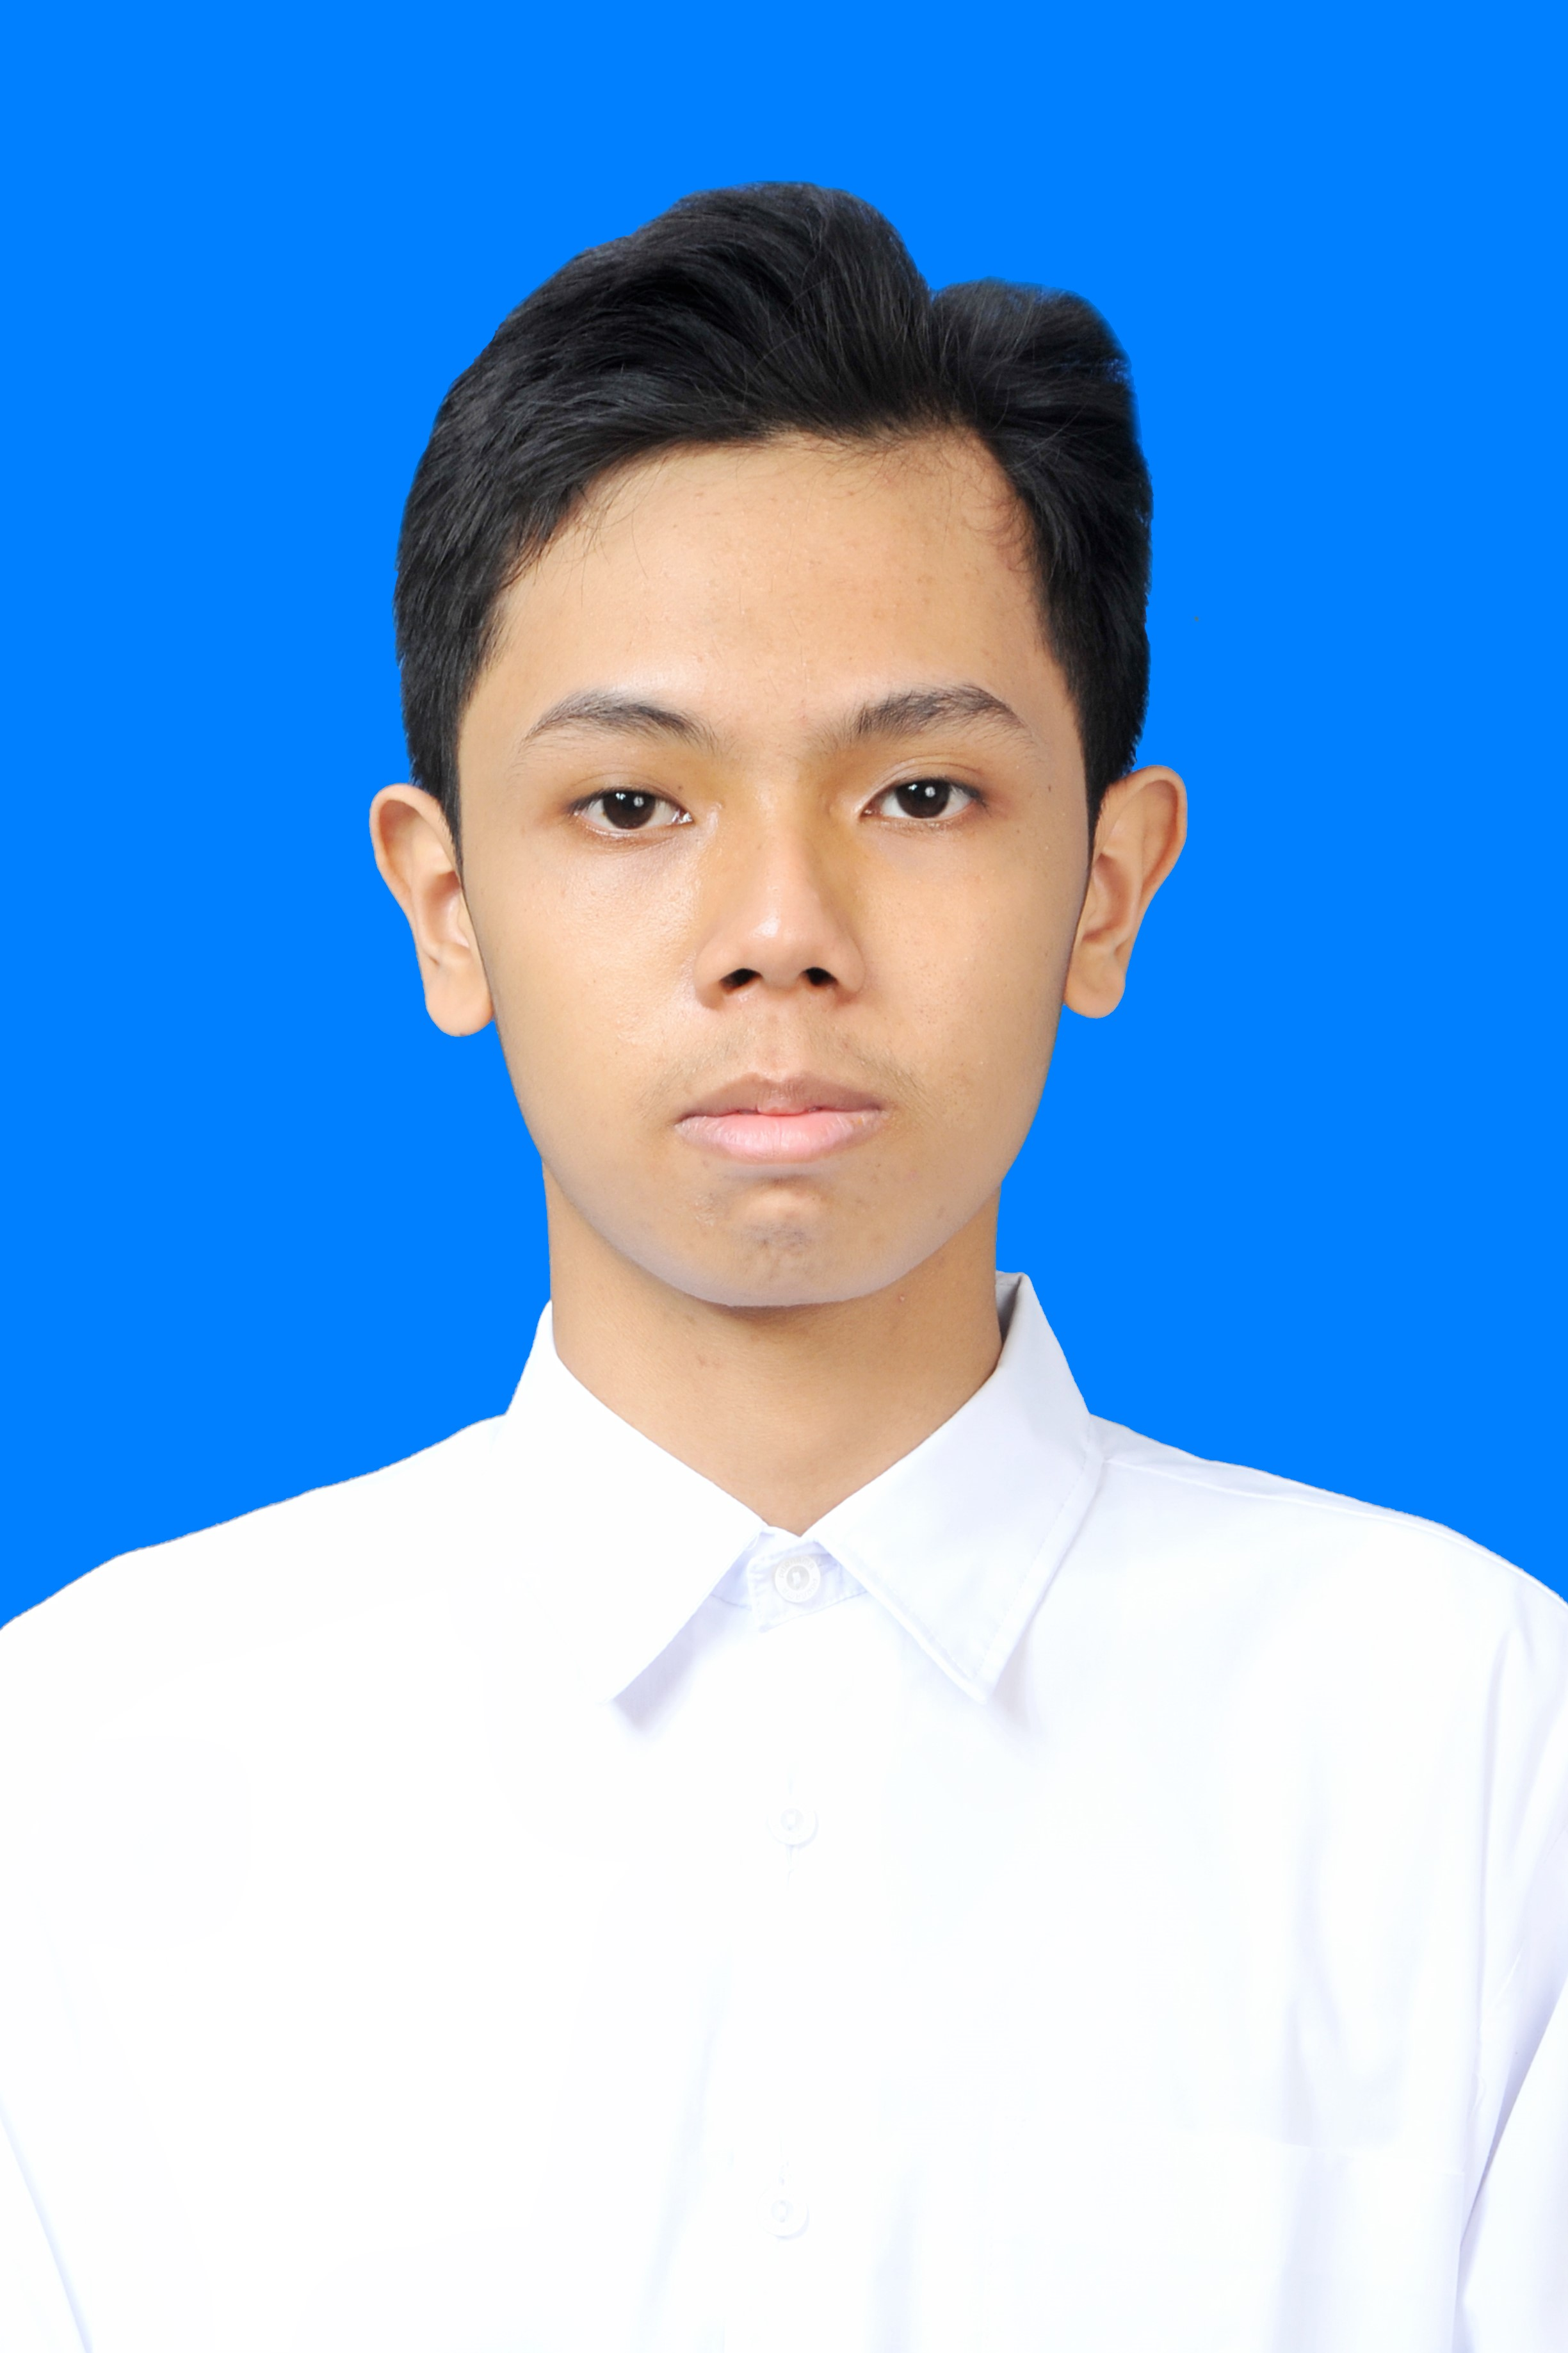
\includegraphics[width=0.3\textwidth]{gambar/biografi/gilang.jpg}
  \vspace{-4ex}
\end{wrapfigure}

% Ubah kalimat berikut dengan biografi dari mahasiswa
\name{}, atau yang biasa dikenal dengan Gilang, lahir pada tanggal 30 Mei 2002 di kota Tuban. Penulis merupakan anak kedua dari dua bersaudara yang tinggal dan besar di Tuban, Jawa Timur. Setelah lulus dari SMA Negeri 1 Tuban, penulis kemudian melanjutkan pendidikan ke jenjang strata satu di Departemen Teknik Komputer, Fakultas Teknologi Elektro dan Informatika Cerdas, Institut Teknologi Sepuluh Nopember mulai tahun 2020.

Penulis merupakan orang yang aktif berorganisasi, dan memiliki berbagai \emph{softskill} serta \emph{hardskill}. Hal ini dibuktikan dengan rekam jejak organisasi dan kepanitiaan dari penulis seperti, Wakil Kepala Departemen Hubungan Luar Himpunan Mahasiswa Teknik Komputer ITS (HIMATEKKOM-ITS), Wakil Ketua Divisi Desain dan Dokumentasi \emph{Multimedia and Game Event}, Ketua Capstone Project pada Bangkit Academy yang diselenggarakan oleh Google, Cloud Engineer pada Bangkit Academy Capstone project, dan masih banyak lagi.